\chapter{Behaviors}\label{c:behave}
In the last chapter we developed a controller for simultaneously regulating the speed and heading of our direct-drive robot model.  Figure~\ref{f:uni_fdbk} illustrates how we might visualize this type of controller.
\begin{figure}[hbt]
\centering
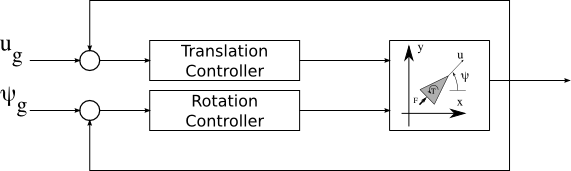
\includegraphics[width=\FigWidth\textwidth]{uni_fdbk.png}
\caption{Simultaneous, independent control for translation and rotation.}
\label{f:uni_fdbk}
\end{figure}
The reasons this approach works so well is that dynamics of our system are such that the system states we are controlling ($u(t)$ and $\psi(t)$) uncoupled, i.e., the forward speed and heading are independent, and the inputs to the system ($F(t)$ and $T(t)$) affect these states independently.  With this kind of scenario we can be fairly confident that sequential loop closure will result a reasonable stability and performance.

In this chapter we'll develop two examples of behavior controllers where we want to achieve something (going to a waypoint or following a line) that requires that we coordinate our inputs, i.e., our goal state is dependent on both control inputs in coupled manner.  One way to approach this kind of problem is illustrated in Figure~\ref{f:uni_fdbk_behave} were we still have our independent translation and rotation controllers, but we've added a higher-level controller that provides continually varying setpoints to these low-level controllers.
\begin{figure}[hbt]
\centering
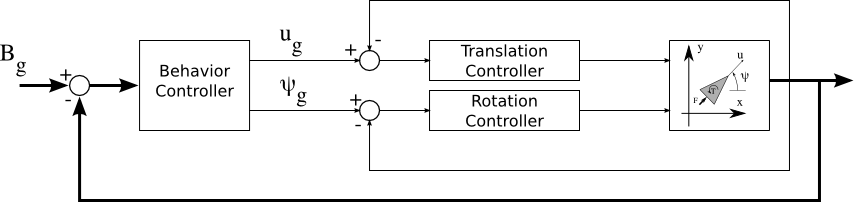
\includegraphics[width=\FigWidth\textwidth]{uni_fdbk_behave.png}
\caption{Behavior control approach.  The high-level Behavior Controller supplies continually varying setpoints to the two low-level controllers for translation and rotation.}
\label{f:uni_fdbk_behave}
\end{figure}


\section{Waypoint Control}
Often we would like to control the position of a mobile robot, giving it commands that consist of a sequential list of waypoints to achieve.  Figure~\ref{f:waypoint} illustrates this scenario with our horizontal, direct-drive robot model.  Our challenge is to design a control algorithm for the force ($F$) and torque ($T$) inputs that will minimize the error between the robot position $(x,y)$ and the waypoint position $(x_1,y_1)$.  

\begin{figure}[hbt]
\centering
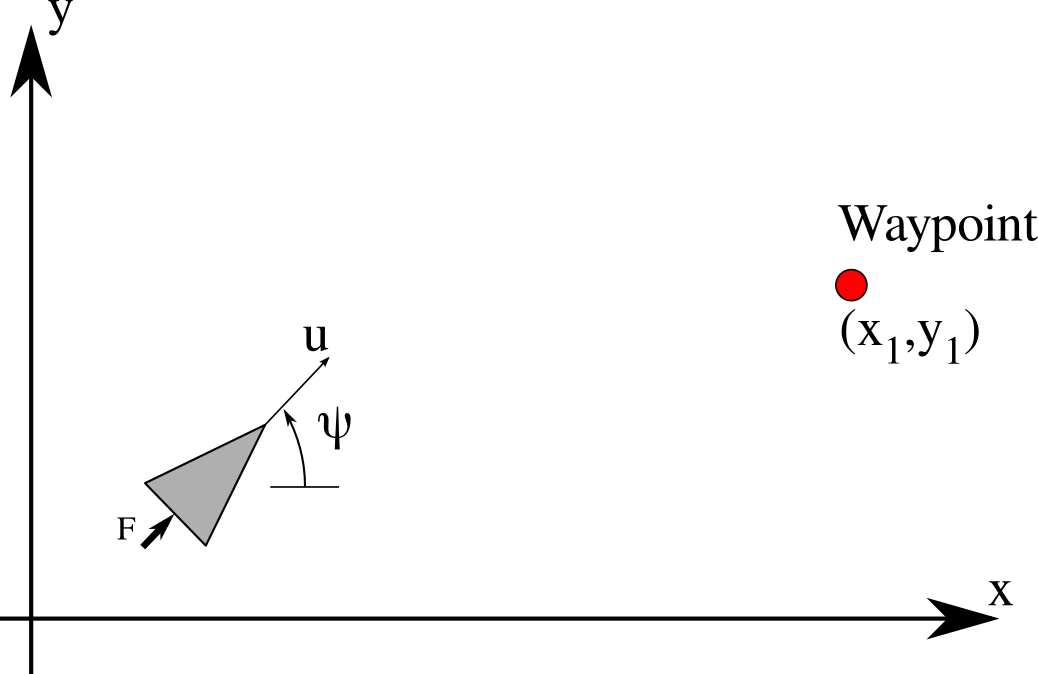
\includegraphics[width=\FigWidth\textwidth]{uni_model_waypoint.png}
\caption{Waypoint}
\label{f:waypoint}
\end{figure}

There are many ways to solve this problem.  Some of these solutions might minimize the time taken to get to the waypoint, minimize the total energy used, etc.  Here we present a simple, but useful waypoint control approach that makes use of our previous work on controlling the heading and velocity.  Keep in mind this is just one of many solutions.
\begin{itemize}
\item Calculate the angle from the current robot position to the waypoint: $\psi_{\mathrm{goal}}$
\item Regulate the heading to achieve $\psi_{\mathrm{goal}}$, i.e., $\psi_{\mathrm{goal}}$ is the setpoint for a heading controller that determines the torque applied to the robot model.
\item Calculate the distance from the current robot position the waypoint: $d_{\mathrm{goal}}$
\item If we are far from the waypoint ($d_{\mathrm{goal}} > R$) 
  \begin{itemize}
  \item Regulate the speed to achieve $u_{\mathrm{goal}}$
  \end{itemize}
\item  If we are close the waypoint ($d_{\mathrm{goal}} \leq R$) 
  \begin{itemize}
  \item Regulate the distance to minimize the distance from the waypoint
  \end{itemize}
\item If we are very close to the waypoint ($d_{\mathrm{goal}} \leq S$) 
  \begin{itemize}
  \item Declare the waypoint 'achieved' and move on to the next waypoint.
  \end{itemize}
\end{itemize}

\[
d_{\mathrm{goal}}=\sqrt{\left(x_1-x\right)^2 + \left(y_1-y\right)^2}
\]

\[
\psi_{\mathrm{goal}}=\arctan{\frac{y_1-y}{x_1-x}}
\]
A common mistake in calculating $\psi_{\mathrm{goal}}$ is to not properly consider all for possible quadrants.  Most computational platforms have a function \texttt{atan2(Y,X)} that returns an angle in the appropriate quadrant.

\begin{figure}[hbt]
\centering
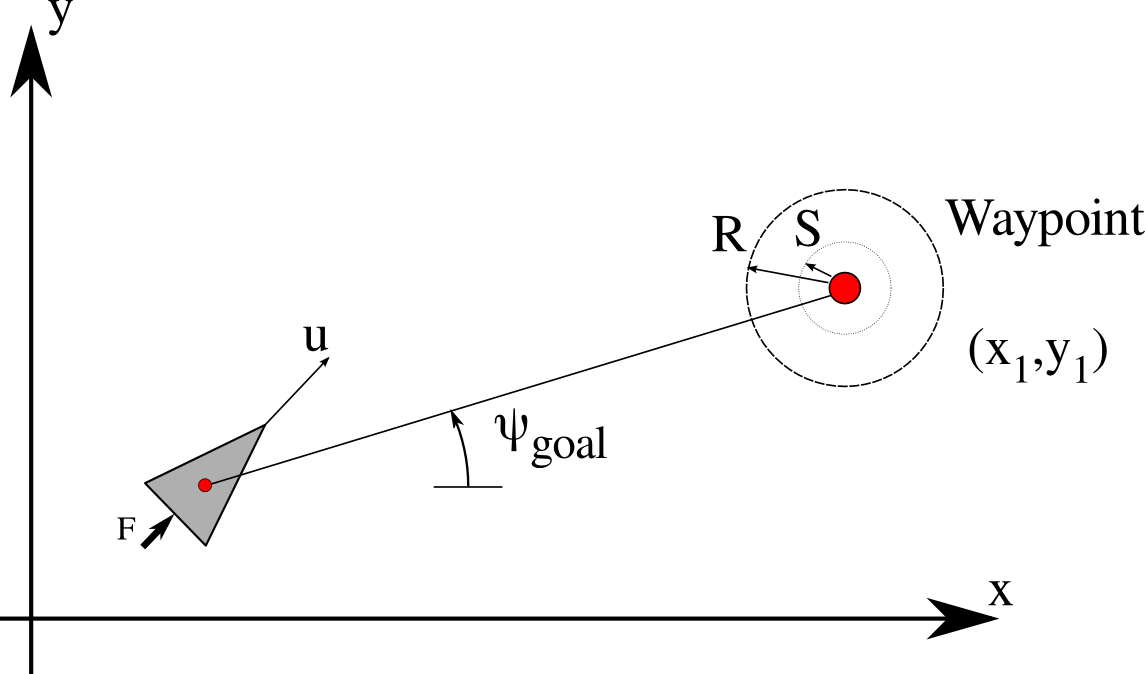
\includegraphics[width=\FigWidth\textwidth]{uni_model_waypoint_annote.png}
\caption{Waypoint}
\label{f:waypoint_annote}
\end{figure}

\begin{ex}
Building on the heading/speed controller you developed in Exercise~\ref{ex:state_cntrl}, develop a waypoint controller.  The goal is to start with all six initial states at zero and control the direct-drive robot model to reach a final waypoint of $(x=25,y=35)$ at a speed of \unitfrac[1.0]{m}{s}.  (You may want to slow down as you get close to the waypoint!)  Your governing equations, model parameters and thrust/torque limits should be the same as stated in Exercise~\ref{ex:state_cntrl}.  You can declare success---waypoint achieved---when the robot gets within \unit[0.5]{m} of the given final waypoint.

Submit the following:
\begin{itemize}
\item A graph of the x-y position reported by your model for the waypoint control simulation.
\item Graphs of the states of your model as a function of time for waypoint control.
\item A discussion of what is pertinent in the graphs - what do you observe that makes you think the simulation and controllers are acting appropriately?
\end{itemize}
\end{ex}


\section{Line Following---Line-of-Sight Control}
A waypoint controller attempts to achieve a final state---the waypoint position---without specifying how we get there.  A line following controller attempts to achieve a final state---the end of the line---but also specifies the path to take to get to that point.  (Line following is a specific example of a more general \emph{path following} controller.)  Figure~\ref{f:line} illustrates this scenario where we'd like our direct-drive robot model to follow the line described by the two endpoints, ending up at the final point $(x_2,y_2)$.

\begin{figure}[hbt]
\centering
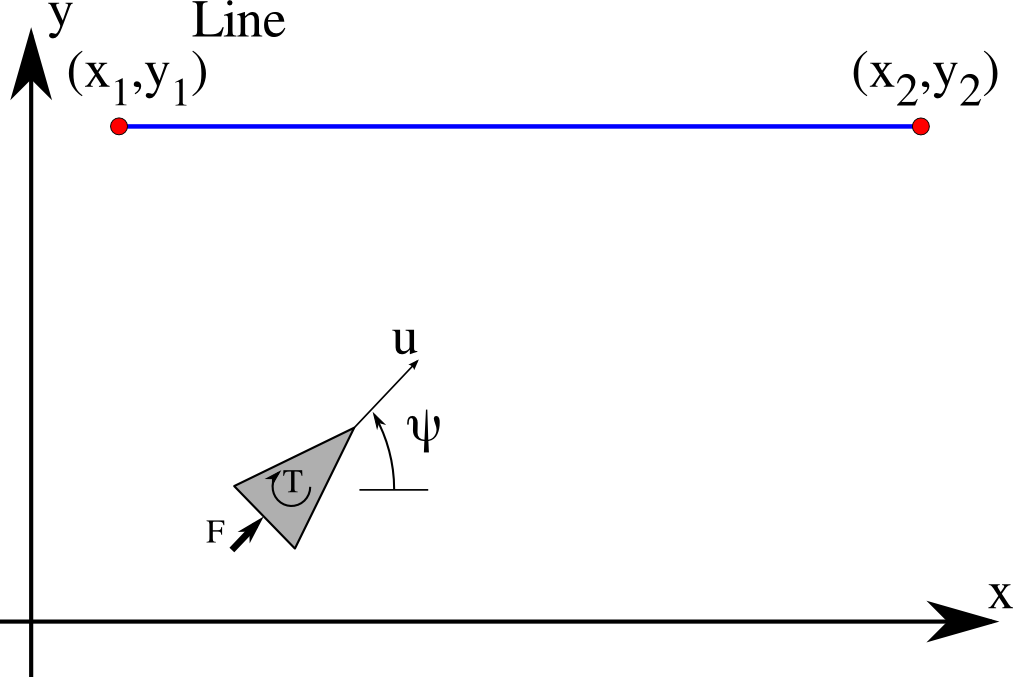
\includegraphics[width=\FigWidth\textwidth]{uni_model_line.png}
\caption{Line following}
\label{f:line}
\end{figure}

There are many ways to solve this type of problem.  One control behavior that works well for following linear features is the \emph{line-of-sight} (LOS) algorithm.  The basic concept is as follows:
\begin{itemize}
\item Given the endpoints of the line-to-follow and the current position of the robot, calculate the shortest distance to the line.  This can be done by defining a line perpendicular to the line-to-follow and the solving for the intersection of the two lines: $(x_i,y_i)$.
\item Find the point along the line-to-follow a fixed \emph{look ahead distance} ($d_{\mathrm{LOS}}$) from $(x_i,y_i)$ towards the goal point $(x_2,y_2)$.  This point is $(x_L,y_L)$.
\item Calculate the heading goal as the angle from the current location to $(x_L,y_L)$.
\item Use the translation (speed) and rotation (heading) controllers to move the robot towards $(x_L,y_L)$ at a given speed.
\end{itemize}
This geometry is illustrated in Figure~\ref{f:line_geo}.
\begin{figure}[hbt]
\centering
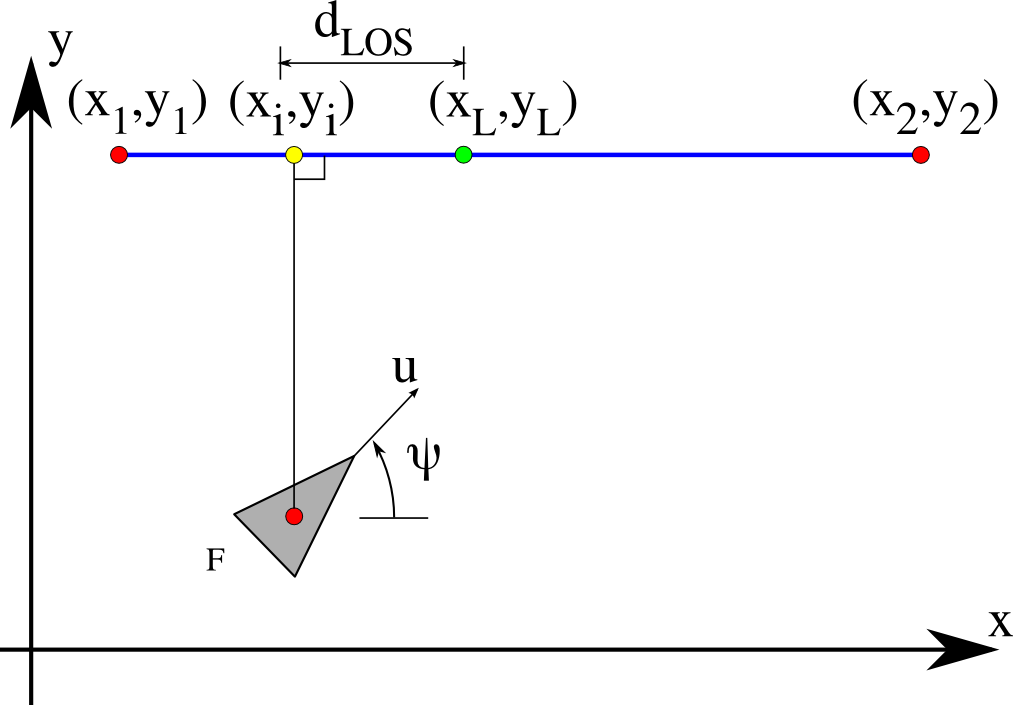
\includegraphics[width=\FigWidth\textwidth]{uni_model_line_geo.png}
\caption{Line following}
\label{f:line_geo}
\end{figure}

\subsection{LOS Geometry}

Slope of the line
\[
m = \frac{y_2-y_1}{x_2-x_1}
\]

Intersection point
\begin{align}\label{e:intersection}
x_i & = \frac{m}{m^2+1}\left(y-y_1+m(x_1)+\frac{x}{m}\right) \nonumber \\
y_i & = y_1+m(x_i-x_1) 
\end{align}

\begin{ex}
Derive the expressions in (\ref{e:intersection}) given the current position $(x,y)$ and the endpoints of the line $(x_1,y_1)$ and $(x_2,y_2)$.  You might recall that two perpendicular lines have slopes that are negative reciprocals of each other.
\end{ex}

\begin{ex}
The expression for the intersection point (\ref{e:intersection} does not hold if the slope ($m$) is zero or infinity.
\begin{itemize}
\item If $m=0$ (horizontal line), provide expressions for $x_i$ and $y_i$ given the current position $(x,y)$ and the endpoints of the line $(x_1,y_1)$ and $(x_2,y_2)$.
\item If $m=\infty$ (vertical line), provide expressions for $x_i$ and $y_i$ given the current position $(x,y)$ and the endpoints of the line $(x_1,y_1)$ and $(x_2,y_2)$.
\end{itemize}
\end{ex}



